\documentclass[]{article}
\usepackage{lmodern}
\usepackage{amssymb,amsmath}
\usepackage{ifxetex,ifluatex}
\usepackage{fixltx2e} % provides \textsubscript
\ifnum 0\ifxetex 1\fi\ifluatex 1\fi=0 % if pdftex
  \usepackage[T1]{fontenc}
  \usepackage[utf8]{inputenc}
\else % if luatex or xelatex
  \ifxetex
    \usepackage{mathspec}
  \else
    \usepackage{fontspec}
  \fi
  \defaultfontfeatures{Ligatures=TeX,Scale=MatchLowercase}
\fi
% use upquote if available, for straight quotes in verbatim environments
\IfFileExists{upquote.sty}{\usepackage{upquote}}{}
% use microtype if available
\IfFileExists{microtype.sty}{%
\usepackage{microtype}
\UseMicrotypeSet[protrusion]{basicmath} % disable protrusion for tt fonts
}{}
\usepackage[margin=1in]{geometry}
\usepackage{hyperref}
\hypersetup{unicode=true,
            pdftitle={Running multiple analyses at once using the CaseCrossover package},
            pdfauthor={Martijn J. Schuemie},
            pdfborder={0 0 0},
            breaklinks=true}
\urlstyle{same}  % don't use monospace font for urls
\usepackage{color}
\usepackage{fancyvrb}
\newcommand{\VerbBar}{|}
\newcommand{\VERB}{\Verb[commandchars=\\\{\}]}
\DefineVerbatimEnvironment{Highlighting}{Verbatim}{commandchars=\\\{\}}
% Add ',fontsize=\small' for more characters per line
\usepackage{framed}
\definecolor{shadecolor}{RGB}{248,248,248}
\newenvironment{Shaded}{\begin{snugshade}}{\end{snugshade}}
\newcommand{\AlertTok}[1]{\textcolor[rgb]{0.94,0.16,0.16}{#1}}
\newcommand{\AnnotationTok}[1]{\textcolor[rgb]{0.56,0.35,0.01}{\textbf{\textit{#1}}}}
\newcommand{\AttributeTok}[1]{\textcolor[rgb]{0.77,0.63,0.00}{#1}}
\newcommand{\BaseNTok}[1]{\textcolor[rgb]{0.00,0.00,0.81}{#1}}
\newcommand{\BuiltInTok}[1]{#1}
\newcommand{\CharTok}[1]{\textcolor[rgb]{0.31,0.60,0.02}{#1}}
\newcommand{\CommentTok}[1]{\textcolor[rgb]{0.56,0.35,0.01}{\textit{#1}}}
\newcommand{\CommentVarTok}[1]{\textcolor[rgb]{0.56,0.35,0.01}{\textbf{\textit{#1}}}}
\newcommand{\ConstantTok}[1]{\textcolor[rgb]{0.00,0.00,0.00}{#1}}
\newcommand{\ControlFlowTok}[1]{\textcolor[rgb]{0.13,0.29,0.53}{\textbf{#1}}}
\newcommand{\DataTypeTok}[1]{\textcolor[rgb]{0.13,0.29,0.53}{#1}}
\newcommand{\DecValTok}[1]{\textcolor[rgb]{0.00,0.00,0.81}{#1}}
\newcommand{\DocumentationTok}[1]{\textcolor[rgb]{0.56,0.35,0.01}{\textbf{\textit{#1}}}}
\newcommand{\ErrorTok}[1]{\textcolor[rgb]{0.64,0.00,0.00}{\textbf{#1}}}
\newcommand{\ExtensionTok}[1]{#1}
\newcommand{\FloatTok}[1]{\textcolor[rgb]{0.00,0.00,0.81}{#1}}
\newcommand{\FunctionTok}[1]{\textcolor[rgb]{0.00,0.00,0.00}{#1}}
\newcommand{\ImportTok}[1]{#1}
\newcommand{\InformationTok}[1]{\textcolor[rgb]{0.56,0.35,0.01}{\textbf{\textit{#1}}}}
\newcommand{\KeywordTok}[1]{\textcolor[rgb]{0.13,0.29,0.53}{\textbf{#1}}}
\newcommand{\NormalTok}[1]{#1}
\newcommand{\OperatorTok}[1]{\textcolor[rgb]{0.81,0.36,0.00}{\textbf{#1}}}
\newcommand{\OtherTok}[1]{\textcolor[rgb]{0.56,0.35,0.01}{#1}}
\newcommand{\PreprocessorTok}[1]{\textcolor[rgb]{0.56,0.35,0.01}{\textit{#1}}}
\newcommand{\RegionMarkerTok}[1]{#1}
\newcommand{\SpecialCharTok}[1]{\textcolor[rgb]{0.00,0.00,0.00}{#1}}
\newcommand{\SpecialStringTok}[1]{\textcolor[rgb]{0.31,0.60,0.02}{#1}}
\newcommand{\StringTok}[1]{\textcolor[rgb]{0.31,0.60,0.02}{#1}}
\newcommand{\VariableTok}[1]{\textcolor[rgb]{0.00,0.00,0.00}{#1}}
\newcommand{\VerbatimStringTok}[1]{\textcolor[rgb]{0.31,0.60,0.02}{#1}}
\newcommand{\WarningTok}[1]{\textcolor[rgb]{0.56,0.35,0.01}{\textbf{\textit{#1}}}}
\usepackage{graphicx,grffile}
\makeatletter
\def\maxwidth{\ifdim\Gin@nat@width>\linewidth\linewidth\else\Gin@nat@width\fi}
\def\maxheight{\ifdim\Gin@nat@height>\textheight\textheight\else\Gin@nat@height\fi}
\makeatother
% Scale images if necessary, so that they will not overflow the page
% margins by default, and it is still possible to overwrite the defaults
% using explicit options in \includegraphics[width, height, ...]{}
\setkeys{Gin}{width=\maxwidth,height=\maxheight,keepaspectratio}
\IfFileExists{parskip.sty}{%
\usepackage{parskip}
}{% else
\setlength{\parindent}{0pt}
\setlength{\parskip}{6pt plus 2pt minus 1pt}
}
\setlength{\emergencystretch}{3em}  % prevent overfull lines
\providecommand{\tightlist}{%
  \setlength{\itemsep}{0pt}\setlength{\parskip}{0pt}}
\setcounter{secnumdepth}{5}
% Redefines (sub)paragraphs to behave more like sections
\ifx\paragraph\undefined\else
\let\oldparagraph\paragraph
\renewcommand{\paragraph}[1]{\oldparagraph{#1}\mbox{}}
\fi
\ifx\subparagraph\undefined\else
\let\oldsubparagraph\subparagraph
\renewcommand{\subparagraph}[1]{\oldsubparagraph{#1}\mbox{}}
\fi

%%% Use protect on footnotes to avoid problems with footnotes in titles
\let\rmarkdownfootnote\footnote%
\def\footnote{\protect\rmarkdownfootnote}

%%% Change title format to be more compact
\usepackage{titling}

% Create subtitle command for use in maketitle
\newcommand{\subtitle}[1]{
  \posttitle{
    \begin{center}\large#1\end{center}
    }
}

\setlength{\droptitle}{-2em}

  \title{Running multiple analyses at once using the CaseCrossover package}
    \pretitle{\vspace{\droptitle}\centering\huge}
  \posttitle{\par}
    \author{Martijn J. Schuemie}
    \preauthor{\centering\large\emph}
  \postauthor{\par}
      \predate{\centering\large\emph}
  \postdate{\par}
    \date{2018-11-23}


\begin{document}
\maketitle

{
\setcounter{tocdepth}{2}
\tableofcontents
}
\hypertarget{introduction}{%
\section{Introduction}\label{introduction}}

In this vignette we focus on running several different analyses on
several exposure-outcome-nesting cohort triplets This can be useful when
we want to explore the sensitivity to analyses choices, include
controls, or run an experiment similar to the OMOP experiment to
empirically identify the optimal analysis choices for a particular
research question.

This vignette assumes you are already familiar with the
\texttt{CaseCrossover} package and are able to perform single studies.
We will walk through all the steps needed to perform an exemplar set of
analyses, and we have selected the well-studied topic of the effect of
nonsteroidal anti-inflammatory drugs (NSAIDs) on gastrointestinal (GI)
bleeding-related hospitalization. For simplicity, we focus on one NSAID:
diclofenac. We will execute various variations of an analysis for the
primary exposure pair and a large set of negative control exposures.

\hypertarget{general-approach}{%
\section{General approach}\label{general-approach}}

The general approach to running a set of analyses is that you specify
all the function arguments of the functions you would normally call, and
create sets of these function arguments. The final models as well as
intermediate data objects will all be saved to disk for later
extraction.

An analysis will be executed by calling these functions in sequence:

\begin{enumerate}
\def\labelenumi{\arabic{enumi}.}
\tightlist
\item
  \texttt{getDbCaseCrossoverData()}
\item
  \texttt{selectSubjectsToInclude()}
\item
  \texttt{getExposureStatus()}
\item
  \texttt{fitCaseCrossoverModel()}
\end{enumerate}

When you provide several analyses to the \texttt{CaseCrossover} package,
it will determine whether any of the analyses and
exposure-outcome-nesting triplets cohort triplets have anything in
common, and will take advantage of this fact. For example, if we specify
several exposure-outcome-nesting triplets with the same outcome and
nesting cohort, the data for the cases will be extracted only once.

The function arguments you need to define have been divided into four
groups:

\begin{enumerate}
\def\labelenumi{\arabic{enumi}.}
\tightlist
\item
  \textbf{Hypothesis of interest}: arguments that are specific to a
  hypothesis of interest, in the case of the case-crossover design this
  is a combination of exposure, outcome, and optionally a cohort in
  which the analysis is nested.
\item
  \textbf{Analyses}: arguments that are not directly specific to a
  hypothesis of interest, such as the washout window, whether to focus
  on first outcomes or all, or whether to adjust for time trends in
  exposure.
\item
  Arguments that are the output of a previous function in the
  \texttt{CaseCrossover} package, such as the \texttt{caseCrossoverData}
  argument of the \texttt{selectSubjectsToInclude} function. These
  cannot be specified by the user.
\item
  Arguments that are specific to an environment, such as the connection
  details for connecting to the server, and the name of the schema
  holding the CDM data.
\end{enumerate}

\hypertarget{preparation-for-the-example}{%
\section{Preparation for the
example}\label{preparation-for-the-example}}

We need to tell R how to connect to the server where the data are.
\texttt{CaseCrossover} uses the \texttt{DatabaseConnector} package,
which provides the \texttt{createConnectionDetails} function. Type
\texttt{?createConnectionDetails} for the specific settings required for
the various database management systems (DBMS). For example, one might
connect to a PostgreSQL database using this code:

\begin{Shaded}
\begin{Highlighting}[]
\NormalTok{connectionDetails <-}\StringTok{ }\KeywordTok{createConnectionDetails}\NormalTok{(}\DataTypeTok{dbms =} \StringTok{"postgresql"}\NormalTok{, }
                                             \DataTypeTok{server =} \StringTok{"localhost/ohdsi"}\NormalTok{, }
                                             \DataTypeTok{user =} \StringTok{"joe"}\NormalTok{, }
                                             \DataTypeTok{password =} \StringTok{"supersecret"}\NormalTok{)}

\NormalTok{outputFolder <-}\StringTok{ "/home/ccrOutput"}

\NormalTok{cdmDatabaseSchema <-}\StringTok{ "my_cdm_data"}
\NormalTok{cohortDatabaseSchema <-}\StringTok{ "my_work_schema"}
\NormalTok{cohortTable <-}\StringTok{ "vignette_cohorts"}
\end{Highlighting}
\end{Shaded}

The last two lines define the \texttt{cdmDatabaseSchema} and
\texttt{cohortDatabaseSchema} variables. We'll use these later to tell R
where the data in CDM format live, and where we want to store the
outcome and nesting cohorts. Note that for Microsoft SQL Server,
databaseschemas need to specify both the database and the schema, so for
example \texttt{cdmDatabaseSchema\ \textless{}-\ "my\_cdm\_data.dbo"}.

We also need to prepare our exposures, outcomes and nesting cohorts of
interest. The \texttt{drug\_era} table in the OMOP Common Data Model
already contains prespecified cohorts of users at the ingredient level,
so we will use that for the exposures here. Note that we can also use
custom-defined exposure cohorts, such as those created in ATLAS. For the
outcomes, we want to restrict our analysis only to those events that are
recorded in an inpatient setting, so we will need to create a custom
cohort table. For this example, we are only interested in GI bleed
(concept ID 192671). Some of the analyses we'd like to nest in a
population with previous diagnoses of rheumatoid arthritis, so we will
need to create a custom cohort for this as well.

We create a text file called \emph{vignette.sql} with the following
content:

\begin{Shaded}
\begin{Highlighting}[]
\CommentTok{/***********************************}
\CommentTok{File vignette.sql }
\CommentTok{***********************************/}

\KeywordTok{IF}\NormalTok{ OBJECT_ID(}\StringTok{'@cohortDatabaseSchema.@cohortTable'}\NormalTok{, }\StringTok{'U'}\NormalTok{) }\KeywordTok{IS} \KeywordTok{NOT} \KeywordTok{NULL}
  \KeywordTok{DROP} \KeywordTok{TABLE}\NormalTok{ @cohortDatabaseSchema.@cohortTable;}

\KeywordTok{SELECT} \DecValTok{1} \KeywordTok{AS}\NormalTok{ cohort_definition_id,}
\NormalTok{    condition_start_date }\KeywordTok{AS}\NormalTok{ cohort_start_date,}
\NormalTok{    condition_end_date }\KeywordTok{AS}\NormalTok{ cohort_end_date,}
\NormalTok{    condition_occurrence.person_id }\KeywordTok{AS}\NormalTok{ subject_id}
\KeywordTok{INTO}\NormalTok{ @cohortDatabaseSchema.@cohortTable}
\KeywordTok{FROM}\NormalTok{ @cdmDatabaseSchema.condition_occurrence}
\KeywordTok{INNER} \KeywordTok{JOIN}\NormalTok{ @cdmDatabaseSchema.visit_occurrence}
    \KeywordTok{ON}\NormalTok{ condition_occurrence.visit_occurrence_id = visit_occurrence.visit_occurrence_id}
\KeywordTok{WHERE}\NormalTok{ condition_concept_id }\KeywordTok{IN}\NormalTok{ (}
        \KeywordTok{SELECT}\NormalTok{ descendant_concept_id}
        \KeywordTok{FROM}\NormalTok{ @cdmDatabaseSchema.concept_ancestor}
        \KeywordTok{WHERE}\NormalTok{ ancestor_concept_id = }\DecValTok{192671} \CommentTok{-- GI - Gastrointestinal haemorrhage}
\NormalTok{        )}
    \KeywordTok{AND}\NormalTok{ visit_occurrence.visit_concept_id }\KeywordTok{IN}\NormalTok{ (}\DecValTok{9201}\NormalTok{, }\DecValTok{9203}\NormalTok{);}
    
\KeywordTok{INSERT} \KeywordTok{INTO}\NormalTok{ @cohortDatabaseSchema.@cohortTable }
\NormalTok{(cohort_definition_id, cohort_start_date, cohort_end_date, subject_id)}
\KeywordTok{SELECT} \DecValTok{2} \KeywordTok{AS}\NormalTok{ cohort_definition_id,}
    \FunctionTok{MIN}\NormalTok{(condition_start_date) }\KeywordTok{AS}\NormalTok{ cohort_start_date,}
    \KeywordTok{NULL} \KeywordTok{AS}\NormalTok{ cohort_end_date,}
\NormalTok{    person_id }\KeywordTok{AS}\NormalTok{ subject_id}
\KeywordTok{FROM}\NormalTok{ @cdmDatabaseSchema.condition_occurrence}
\KeywordTok{WHERE}\NormalTok{ condition_concept_id }\KeywordTok{IN}\NormalTok{ (}
        \KeywordTok{SELECT}\NormalTok{ descendant_concept_id}
        \KeywordTok{FROM}\NormalTok{ @cdmDatabaseSchema.concept_ancestor}
        \KeywordTok{WHERE}\NormalTok{ ancestor_concept_id = }\DecValTok{80809} \CommentTok{-- rheumatoid arthritis}
\NormalTok{        )}
\KeywordTok{GROUP} \KeywordTok{BY}\NormalTok{ person_id;}
\end{Highlighting}
\end{Shaded}

This is parameterized SQL which can be used by the \texttt{SqlRender}
package. We use parameterized SQL so we do not have to pre-specify the
names of the CDM and result schemas. That way, if we want to run the SQL
on a different schema, we only need to change the parameter values; we
do not have to change the SQL code. By also making use of translation
functionality in \texttt{SqlRender}, we can make sure the SQL code can
be run in many different environments.

\begin{Shaded}
\begin{Highlighting}[]
\KeywordTok{library}\NormalTok{(SqlRender)}
\NormalTok{sql <-}\StringTok{ }\KeywordTok{readSql}\NormalTok{(}\StringTok{"vignette.sql"}\NormalTok{)}
\NormalTok{sql <-}\StringTok{ }\KeywordTok{renderSql}\NormalTok{(sql,}
                 \DataTypeTok{cdmDatabaseSchema =}\NormalTok{ cdmDatabaseSchema, }
                 \DataTypeTok{cohortDatabaseSchema =}\NormalTok{ cohortDatabaseSchema,}
                 \DataTypeTok{cohortTable =}\NormalTok{ cohortTable)}\OperatorTok{$}\NormalTok{sql}
\NormalTok{sql <-}\StringTok{ }\KeywordTok{translateSql}\NormalTok{(sql, }\DataTypeTok{targetDialect =}\NormalTok{ connectionDetails}\OperatorTok{$}\NormalTok{dbms)}\OperatorTok{$}\NormalTok{sql}

\NormalTok{connection <-}\StringTok{ }\KeywordTok{connect}\NormalTok{(connectionDetails)}
\KeywordTok{executeSql}\NormalTok{(connection, sql)}
\end{Highlighting}
\end{Shaded}

In this code, we first read the SQL from the file into memory. In the
next line, we replace the two parameter names with the actual values. We
then translate the SQL into the dialect appropriate for the DBMS we
already specified in the \texttt{connectionDetails}. Next, we connect to
the server, and submit the rendered and translated SQL.

\hypertarget{specifying-hypotheses-of-interest}{%
\section{Specifying hypotheses of
interest}\label{specifying-hypotheses-of-interest}}

The first group of arguments define the exposure, outcome, and
optionally the nesting cohort. Here we demonstrate how to create a list
of exposure-outcome-nesting cohort triplets:

\begin{Shaded}
\begin{Highlighting}[]
\NormalTok{negativeControls <-}\StringTok{ }\KeywordTok{c}\NormalTok{(}\DecValTok{705178}\NormalTok{,}
                      \DecValTok{705944}\NormalTok{,}
                      \DecValTok{710650}\NormalTok{,}
                      \DecValTok{714785}\NormalTok{,}
                      \DecValTok{719174}\NormalTok{,}
                      \DecValTok{719311}\NormalTok{,}
                      \DecValTok{735340}\NormalTok{,}
                      \DecValTok{742185}\NormalTok{,}
                      \DecValTok{780369}\NormalTok{,}
                      \DecValTok{781182}\NormalTok{,}
                      \DecValTok{924724}\NormalTok{,}
                      \DecValTok{990760}\NormalTok{,}
                      \DecValTok{1110942}\NormalTok{,}
                      \DecValTok{1111706}\NormalTok{,}
                      \DecValTok{1136601}\NormalTok{,}
                      \DecValTok{1317967}\NormalTok{,}
                      \DecValTok{1501309}\NormalTok{,}
                      \DecValTok{1505346}\NormalTok{,}
                      \DecValTok{1551673}\NormalTok{,}
                      \DecValTok{1560278}\NormalTok{,}
                      \DecValTok{1584910}\NormalTok{,}
                      \DecValTok{19010309}\NormalTok{,}
                      \DecValTok{40163731}\NormalTok{)}
\NormalTok{diclofenac <-}\StringTok{ }\DecValTok{1124300}
\NormalTok{giBleed <-}\StringTok{ }\DecValTok{1}
\NormalTok{rheumatoidArthritis <-}\StringTok{ }\DecValTok{2}

\NormalTok{exposureOutcomeNcList <-}\StringTok{ }\KeywordTok{list}\NormalTok{()}
\ControlFlowTok{for}\NormalTok{ (exposureId }\ControlFlowTok{in} \KeywordTok{c}\NormalTok{(diclofenac, negativeControls)) \{}
\NormalTok{  exposureOutcomeNc <-}\StringTok{ }\KeywordTok{createExposureOutcomeNestingCohort}\NormalTok{(}\DataTypeTok{exposureId =}\NormalTok{ exposureId,}
                                                          \DataTypeTok{outcomeId =}\NormalTok{ giBleed,}
                                                          \DataTypeTok{nestingCohortId =}\NormalTok{ rheumatoidArthritis)}
\NormalTok{  exposureOutcomeNcList[[}\KeywordTok{length}\NormalTok{(exposureOutcomeNcList) }\OperatorTok{+}\StringTok{ }\DecValTok{1}\NormalTok{]] <-}\StringTok{ }\NormalTok{exposureOutcomeNc}
\NormalTok{\}}
\end{Highlighting}
\end{Shaded}

We defined the outcome of interest to be the custom cohort with ID 1 we
defined in the SQL above. The exposures include diclofenac (concept ID
1124300) and a large number of negative control exposures. For each
hypothesis we specify the same nesting cohort with ID 2, as defined in
the SQL above.

A convenient way to save \texttt{exposureOutcomeNcList} to file is by
using the \texttt{saveExposureOutcomeNestingCohortList} function, and we
can load it again using the
\texttt{loadExposureOutcomeNestingCohortList} function.

\hypertarget{specifying-analyses}{%
\section{Specifying analyses}\label{specifying-analyses}}

The second group of arguments are not specific to a hypothesis of
interest, and comprise the majority of arguments. For each function that
will be called during the execution of the analyses, a companion
function is available that has (almost) the same arguments. For example,
for the \texttt{getDbCaseCrossoverData()} function there is the
\texttt{createGetDbCaseCrossoverDataArgs()} function. These companion
functions can be used to create the arguments to be used during
execution:

\begin{Shaded}
\begin{Highlighting}[]
\NormalTok{getDbCaseCrossoverDataArgs1 <-}\StringTok{ }\KeywordTok{createGetDbCaseCrossoverDataArgs}\NormalTok{(}\DataTypeTok{useNestingCohort =} \OtherTok{FALSE}\NormalTok{)}

\NormalTok{selectSubjectsToIncludeArgs1 <-}\StringTok{ }\KeywordTok{createSelectSubjectsToIncludeArgs}\NormalTok{(}\DataTypeTok{firstOutcomeOnly =} \OtherTok{FALSE}\NormalTok{,}
                                                                  \DataTypeTok{washoutPeriod =} \DecValTok{180}\NormalTok{)}

\NormalTok{getExposureStatusArgs1 <-}\StringTok{ }\KeywordTok{createGetExposureStatusArgs}\NormalTok{(}\DataTypeTok{firstExposureOnly =} \OtherTok{FALSE}\NormalTok{,}
                                                      \DataTypeTok{riskWindowStart =} \DecValTok{0}\NormalTok{,}
                                                      \DataTypeTok{riskWindowEnd =} \DecValTok{0}\NormalTok{,}
                                                      \DataTypeTok{controlWindowOffsets =} \DecValTok{-30}\NormalTok{)}
\end{Highlighting}
\end{Shaded}

Any argument that is not explicitly specified by the user will assume
the default value specified in the function. Note that in this example,
even though we specified a nesting cohort for each
exposure-outcome-nesting cohort triplet, we have specified
\texttt{useNestingCohort\ =\ FALSE}, meaning we will not nest this
analysis but rather use the entire population to draw cases and
controls.

We can now combine the arguments for the various functions into a single
analysis:

\begin{Shaded}
\begin{Highlighting}[]
\NormalTok{ccrAnalysis1 <-}\StringTok{ }\KeywordTok{createCcrAnalysis}\NormalTok{(}\DataTypeTok{analysisId =} \DecValTok{1}\NormalTok{,}
                                 \DataTypeTok{description =} \StringTok{"Simple case-crossover"}\NormalTok{,}
                                 \DataTypeTok{getDbCaseCrossoverDataArgs =}\NormalTok{ getDbCaseCrossoverDataArgs1,}
                                 \DataTypeTok{selectSubjectsToIncludeArgs =}\NormalTok{ selectSubjectsToIncludeArgs1,}
                                 \DataTypeTok{getExposureStatusArgs =}\NormalTok{ getExposureStatusArgs1)}
\end{Highlighting}
\end{Shaded}

Note that we have assigned an analysis ID (1) to this set of arguments.
We can use this later to link the results back to this specific set of
choices. We also include a short description of the analysis.

We can easily create more analyses, for example by using nesting and
correcting for time trends in exposure (the time-case-control design):

\begin{Shaded}
\begin{Highlighting}[]
\NormalTok{getDbCaseCrossoverDataArgs2 <-}\StringTok{ }\KeywordTok{createGetDbCaseCrossoverDataArgs}\NormalTok{(}\DataTypeTok{useNestingCohort =} \OtherTok{TRUE}\NormalTok{,}
                                                       \DataTypeTok{getTimeControlData =} \OtherTok{TRUE}\NormalTok{,}
                                                       \DataTypeTok{getVisits =} \OtherTok{TRUE}\NormalTok{)}

\NormalTok{ccrAnalysis2 <-}\StringTok{ }\KeywordTok{createCcrAnalysis}\NormalTok{(}\DataTypeTok{analysisId =} \DecValTok{2}\NormalTok{,}
                                \DataTypeTok{description =} \StringTok{"Nested case-crossover"}\NormalTok{,}
                                \DataTypeTok{getDbCaseCrossoverDataArgs =}\NormalTok{ getDbCaseCrossoverDataArgs2,}
                                \DataTypeTok{selectSubjectsToIncludeArgs =}\NormalTok{ selectSubjectsToIncludeArgs1,}
                                \DataTypeTok{getExposureStatusArgs =}\NormalTok{ getExposureStatusArgs1)}

\NormalTok{matchingCriteria1 <-}\StringTok{ }\KeywordTok{createMatchingCriteria}\NormalTok{(}\DataTypeTok{matchOnAge =} \OtherTok{TRUE}\NormalTok{,}
                                           \DataTypeTok{ageCaliper =} \DecValTok{2}\NormalTok{,}
                                           \DataTypeTok{matchOnGender =} \OtherTok{TRUE}\NormalTok{)}

\NormalTok{selectSubjectsToIncludeArgs2 <-}\StringTok{ }\KeywordTok{createSelectSubjectsToIncludeArgs}\NormalTok{(}\DataTypeTok{firstOutcomeOnly =} \OtherTok{FALSE}\NormalTok{,}
                                                                  \DataTypeTok{washoutPeriod =} \DecValTok{180}\NormalTok{,}
                                                                  \DataTypeTok{matchingCriteria =}\NormalTok{ matchingCriteria1)}

\NormalTok{ccrAnalysis3 <-}\StringTok{ }\KeywordTok{createCcrAnalysis}\NormalTok{(}\DataTypeTok{analysisId =} \DecValTok{3}\NormalTok{,}
                                \DataTypeTok{description =} \StringTok{"Nested case-time-control, matching on age and gender"}\NormalTok{,}
                                \DataTypeTok{getDbCaseCrossoverDataArgs =}\NormalTok{ getDbCaseCrossoverDataArgs2,}
                                \DataTypeTok{selectSubjectsToIncludeArgs =}\NormalTok{ selectSubjectsToIncludeArgs2,}
                                \DataTypeTok{getExposureStatusArgs =}\NormalTok{ getExposureStatusArgs1)}

\NormalTok{matchingCriteria2 <-}\StringTok{ }\KeywordTok{createMatchingCriteria}\NormalTok{(}\DataTypeTok{matchOnAge =} \OtherTok{TRUE}\NormalTok{,}
                                            \DataTypeTok{ageCaliper =} \DecValTok{2}\NormalTok{,}
                                            \DataTypeTok{matchOnGender =} \OtherTok{TRUE}\NormalTok{,}
                                            \DataTypeTok{matchOnVisitDate =} \OtherTok{TRUE}\NormalTok{)}

\NormalTok{selectSubjectsToIncludeArgs3 <-}\StringTok{ }\KeywordTok{createSelectSubjectsToIncludeArgs}\NormalTok{(}\DataTypeTok{firstOutcomeOnly =} \OtherTok{FALSE}\NormalTok{,}
                                                                  \DataTypeTok{washoutPeriod =} \DecValTok{180}\NormalTok{,}
                                                                  \DataTypeTok{matchingCriteria =}\NormalTok{ matchingCriteria2)}

\NormalTok{ccrAnalysis4 <-}\StringTok{ }\KeywordTok{createCcrAnalysis}\NormalTok{(}\DataTypeTok{analysisId =} \DecValTok{4}\NormalTok{,}
                                \DataTypeTok{description =} \StringTok{"Nested case-time-control, matching on age, gender, and visit"}\NormalTok{,}
                                \DataTypeTok{getDbCaseCrossoverDataArgs =}\NormalTok{ getDbCaseCrossoverDataArgs2,}
                                \DataTypeTok{selectSubjectsToIncludeArgs =}\NormalTok{ selectSubjectsToIncludeArgs3,}
                                \DataTypeTok{getExposureStatusArgs =}\NormalTok{ getExposureStatusArgs1)}
\end{Highlighting}
\end{Shaded}

These analyses can be combined in a list:

\begin{Shaded}
\begin{Highlighting}[]
\NormalTok{ccrAnalysisList <-}\StringTok{ }\KeywordTok{list}\NormalTok{(ccrAnalysis1, ccrAnalysis2, ccrAnalysis3, ccrAnalysis4)}
\end{Highlighting}
\end{Shaded}

A convenient way to save \texttt{ccrAnalysisList} to file is by using
the \texttt{saveCcrAnalysisList} function, and we can load it again
using the \texttt{loadCcrAnalysisList} function.

\hypertarget{exposure-outcome-and-nesting-cohort-selection-strategies}{%
\subsection{Exposure, outcome, and nesting cohort selection
strategies}\label{exposure-outcome-and-nesting-cohort-selection-strategies}}

Often we would like to evaluate different definitions of the exposure
and/or outcome, or we want to consider different strategies for
identifying the nesting cohort. We could include these by created extra
exposure-outcome-nesting cohort triplets, but that would mean that all
defined analyses would be executed against these variations of the
definitions, and this may not be what we want. Perhaps we would like to
define just a single sensitivity analyses with a different outcome
definition, in which case we could argue that the strategy of selecting
the outcome becomes part of the analysis.

In such a case, we can define the multiple strategies using a list:

\begin{Shaded}
\begin{Highlighting}[]
\NormalTok{outcomeIds =}\StringTok{ }\KeywordTok{list}\NormalTok{(}\DataTypeTok{narrowDefinition =} \DecValTok{1}\NormalTok{,}
                  \DataTypeTok{broadDefinition =} \DecValTok{11}\NormalTok{)}

\NormalTok{exposureOutcomeNc <-}\StringTok{ }\KeywordTok{createExposureOutcomeNestingCohort}\NormalTok{(}\DataTypeTok{exposureId =} \DecValTok{1124300}\NormalTok{,}
                                                        \DataTypeTok{outcomeId =}\NormalTok{ outcomeIds,}
                                                        \DataTypeTok{nestingCohortId =} \DecValTok{2}\NormalTok{)}
\end{Highlighting}
\end{Shaded}

When we specify an analysis, we can then refer to one definition or the
other:

\begin{Shaded}
\begin{Highlighting}[]
\NormalTok{ccrAnalysis1A <-}\StringTok{ }\KeywordTok{createCcrAnalysis}\NormalTok{(}\DataTypeTok{analysisId =} \DecValTok{1}\NormalTok{,}
                                 \DataTypeTok{description =} \StringTok{"Simple case-crossover, using narrow def."}\NormalTok{,}
                                 \DataTypeTok{outcomeType =} \StringTok{"narrowDefinition"}\NormalTok{,}
                                 \DataTypeTok{getDbCaseCrossoverDataArgs =}\NormalTok{ getDbCaseCrossoverDataArgs1,}
                                 \DataTypeTok{selectSubjectsToIncludeArgs =}\NormalTok{ selectSubjectsToIncludeArgs1,}
                                 \DataTypeTok{getExposureStatusArgs =}\NormalTok{ getExposureStatusArgs1)}

\NormalTok{ccrAnalysis1B <-}\StringTok{ }\KeywordTok{createCcrAnalysis}\NormalTok{(}\DataTypeTok{analysisId =} \DecValTok{2}\NormalTok{,}
                                 \DataTypeTok{description =} \StringTok{"Simple case-crossover, using broad def."}\NormalTok{,}
                                 \DataTypeTok{outcomeType =} \StringTok{"broadDefinition"}\NormalTok{,}
                                 \DataTypeTok{getDbCaseCrossoverDataArgs =}\NormalTok{ getDbCaseCrossoverDataArgs1,}
                                 \DataTypeTok{selectSubjectsToIncludeArgs =}\NormalTok{ selectSubjectsToIncludeArgs1,}
                                 \DataTypeTok{getExposureStatusArgs =}\NormalTok{ getExposureStatusArgs1)}

\NormalTok{ccrAnalysisList2 <-}\StringTok{ }\KeywordTok{list}\NormalTok{(ccrAnalysis1A, ccrAnalysis1B)}
\end{Highlighting}
\end{Shaded}

In this example, the first analysis (analysisId = 1) will use cohort
definition 1 as outcome, whilst the second analysis analysis (analysisId
= 2) will use cohort definition 11 as outcome.

The same mechanism can be used to specifiy types for the exposureId and
nestingCohortId.

\hypertarget{executing-multiple-analyses}{%
\section{Executing multiple
analyses}\label{executing-multiple-analyses}}

We can now run the analyses against the hypotheses of interest using the
\texttt{runCcrAnalyses()}function. This function will run all specified
analyses against all hypotheses of interest, meaning that the total
number of outcome models is
\texttt{length(ccrAnalysisList)\ *\ length(exposureOutcomeNcList)}.

\begin{Shaded}
\begin{Highlighting}[]
\NormalTok{result <-}\StringTok{ }\KeywordTok{runCcrAnalyses}\NormalTok{(}\DataTypeTok{connectionDetails =}\NormalTok{ connectionDetails,}
                        \DataTypeTok{cdmDatabaseSchema =}\NormalTok{ cdmDatabaseSchema,}
                        \DataTypeTok{oracleTempSchema =}\NormalTok{ cdmDatabaseSchema,}
                        \DataTypeTok{exposureDatabaseSchema =}\NormalTok{ cdmDatabaseSchema,}
                        \DataTypeTok{exposureTable =} \StringTok{"drug_era"}\NormalTok{,}
                        \DataTypeTok{outcomeDatabaseSchema =}\NormalTok{ cohortDatabaseSchema,}
                        \DataTypeTok{outcomeTable =}\NormalTok{ cohortTable,}
                        \DataTypeTok{nestingCohortDatabaseSchema =}\NormalTok{ cohortDatabaseSchema,}
                        \DataTypeTok{nestingCohortTable =}\NormalTok{ cohortTable,}
                        \DataTypeTok{outputFolder =}\NormalTok{ outputFolder,}
                        \DataTypeTok{exposureOutcomeNestingCohortList =}\NormalTok{ exposureOutcomeNcList,}
                        \DataTypeTok{ccrAnalysisList =}\NormalTok{ ccrAnalysisList,}
                        \DataTypeTok{getDbCaseCrossoverDataThreads =} \DecValTok{1}\NormalTok{,}
                        \DataTypeTok{selectSubjectsToIncludeThreads =} \DecValTok{4}\NormalTok{,}
                        \DataTypeTok{getExposureStatusThreads =} \DecValTok{3}\NormalTok{,}
                        \DataTypeTok{fitCaseCrossoverModelThreads =} \DecValTok{4}\NormalTok{)}
\end{Highlighting}
\end{Shaded}

In the code above, we provide the arguments for connecting to the
database, which schemas and tables to use, as well as the analyses and
hypotheses of interest. The \texttt{outputFolder} specifies where the
outcome models and intermediate files will be written. We also instruct
\texttt{CaseCrossover} to use multiple threads for various stages in the
analyses, meaning these will be executed in parallel on multiple CPUs in
the computer. Multithreading can significantly reduce execution time,
but will require more system resources such as memory and temporary disk
space.

\hypertarget{restarting}{%
\subsection{Restarting}\label{restarting}}

If for some reason the execution was interrupted, you can restart by
re-issuing the \texttt{runCcrAnalyses()} command. Any intermediate and
final products that have already been completed and written to disk will
be skipped.

\hypertarget{retrieving-the-results}{%
\section{Retrieving the results}\label{retrieving-the-results}}

The result of the \texttt{runCcrAnalyses()} is a data frame with one row
per exposure-outcome-nesting cohort-analysis combination. It provides
the file names of the intermediate and end-result files that were
constructed. For example, we can retrieve the fitted model for the
combination of our drug of interest, outcome, and first analysis:

\begin{Shaded}
\begin{Highlighting}[]
\NormalTok{ccrModelFile <-}\StringTok{ }\NormalTok{result}\OperatorTok{$}\NormalTok{modelFile[result}\OperatorTok{$}\NormalTok{exposureId }\OperatorTok{==}\StringTok{ }\DecValTok{1124300} \OperatorTok{&}\StringTok{ }
\StringTok{                                   }\NormalTok{result}\OperatorTok{$}\NormalTok{outcomeId }\OperatorTok{==}\StringTok{ }\DecValTok{1} \OperatorTok{&}
\StringTok{                                   }\NormalTok{result}\OperatorTok{$}\NormalTok{analysisId }\OperatorTok{==}\StringTok{ }\DecValTok{1}\NormalTok{]}
\NormalTok{ccModel <-}\StringTok{ }\KeywordTok{readRDS}\NormalTok{(}\KeywordTok{file.path}\NormalTok{(outputFolder, ccrModelFile))}
\KeywordTok{summary}\NormalTok{(ccrModel)}
\end{Highlighting}
\end{Shaded}

\begin{verbatim}
#> Case-Crossover fitted model
#> Status: OK
#> 
#>           Estimate lower .95 upper .95    logRr seLogRr
#> treatment 1.049705  0.969490  1.136557 0.048509  0.0406
#> 
#> Counts
#>        Cases Controls Control win. (cases) Control win. (controls)
#> Count 455909        0               455909                       0
#>       Exposed case win. (cases) Exposed control win. (cases)
#> Count                      2910                         2851
#>       Exposed case win. (controls) Exposed control win. (controls)
#> Count                            0                               0
\end{verbatim}

Note that some of the file names will appear several times in the table.
For example, analyses 2-4 share the same ccrData object.

We can create a summary of the results using
\texttt{summarizeCcrAnalyses()}:

\begin{Shaded}
\begin{Highlighting}[]
\NormalTok{analysisSum <-}\StringTok{ }\KeywordTok{summarizeCcrAnalyses}\NormalTok{(result, outputFolder)}
\KeywordTok{head}\NormalTok{(analysisSum)}
\end{Highlighting}
\end{Shaded}

\begin{verbatim}
#>   analysisId exposureId nestingCohortId outcomeId        rr    ci95lb
#> 1          1    1124300               2         1 1.0497051 0.9694903
#> 2          1     705178               2         1 0.7076930 0.4851091
#> 3          1     705944               2         1 0.9364407 0.7794752
#> 4          1     710650               2         1 0.6756773 0.4067868
#> 5          1     714785               2         1 1.1434109 0.9674893
#> 6          1     719174               2         1 1.0152964 0.8998162
#>     ci95ub          p  cases controls casesControlWindows
#> 1 1.136557 0.23168883 455909        0              455909
#> 2 1.032406 0.07274233 455909        0              455909
#> 3 1.125015 0.48296337 455909        0              455909
#> 4 1.122307 0.12995570 455909        0              455909
#> 5 1.351321 0.11589880 455909        0              455909
#> 6 1.145597 0.80536171 455909        0              455909
#>   controlsControlWindows exposedCasesCaseWindow exposedCasesControlWindow
#> 1                      0                   2910                      2851
#> 2                      0                    389                       408
#> 3                      0                   1240                      1255
#> 4                      0                    137                       149
#> 5                      0                   2116                      2079
#> 6                      0                   3172                      3164
#>   exposedControlsCaseWindow exposedControlsControlWindow       logRr
#> 1                         0                            0  0.04850930
#> 2                         0                            0 -0.34574489
#> 3                         0                            0 -0.06566910
#> 4                         0                            0 -0.39203974
#> 5                         0                            0  0.13401577
#> 6                         0                            0  0.01518056
#>      seLogRr
#> 1 0.04055895
#> 2 0.19267522
#> 3 0.09360649
#> 4 0.25889573
#> 5 0.08523966
#> 6 0.06160588
\end{verbatim}

This tells us, per exposure-outcome-nesting cohort-analysis combination,
the estimated relative risk and 95\% confidence interval, as well as the
number of cases, controls (for time-case-control), and number of those
that were exposed to the drug in the various windows.

\hypertarget{empirical-calibration}{%
\subsection{Empirical calibration}\label{empirical-calibration}}

Now that we have produced estimates for all outcomes including our
negative controls, we can perform empirical calibration to estimate the
bias of the various analyses included in our study. We will create the
calibration effect plots for every analysis ID. In each plot, the blue
dots represent our negative control exposures, and the yellow diamond
represents our exposure of interest: diclofenac. An unbiased,
well-calibrated analysis should have 95\% of the negative controls
between the dashed lines (ie. 95\% should have p \textgreater{} .05).

\begin{Shaded}
\begin{Highlighting}[]
\KeywordTok{library}\NormalTok{(EmpiricalCalibration)}

\CommentTok{# Analysis 1: Simple case-crossover}
\NormalTok{negCons <-}\StringTok{ }\NormalTok{analysisSum[analysisSum}\OperatorTok{$}\NormalTok{analysisId }\OperatorTok{==}\StringTok{ }\DecValTok{1} \OperatorTok{&}\StringTok{ }\NormalTok{analysisSum}\OperatorTok{$}\NormalTok{exposureId }\OperatorTok{!=}\StringTok{ }\DecValTok{1124300}\NormalTok{, ]}
\NormalTok{ei <-}\StringTok{  }\NormalTok{analysisSum[analysisSum}\OperatorTok{$}\NormalTok{analysisId }\OperatorTok{==}\StringTok{ }\DecValTok{1} \OperatorTok{&}\StringTok{ }\NormalTok{analysisSum}\OperatorTok{$}\NormalTok{exposureId }\OperatorTok{==}\StringTok{ }\DecValTok{1124300}\NormalTok{, ]}
\NormalTok{null <-}\StringTok{ }\KeywordTok{fitNull}\NormalTok{(negCons}\OperatorTok{$}\NormalTok{logRr, negCons}\OperatorTok{$}\NormalTok{seLogRr)}
\KeywordTok{plotCalibrationEffect}\NormalTok{(}\DataTypeTok{logRrNegatives =}\NormalTok{ negCons}\OperatorTok{$}\NormalTok{logRr, }
                      \DataTypeTok{seLogRrNegatives =}\NormalTok{ negCons}\OperatorTok{$}\NormalTok{seLogRr, }
                      \DataTypeTok{logRrPositives =}\NormalTok{ ei}\OperatorTok{$}\NormalTok{logRr, }
                      \DataTypeTok{seLogRrPositives =}\NormalTok{ ei}\OperatorTok{$}\NormalTok{seLogRr, }
\NormalTok{                      null)}
\end{Highlighting}
\end{Shaded}

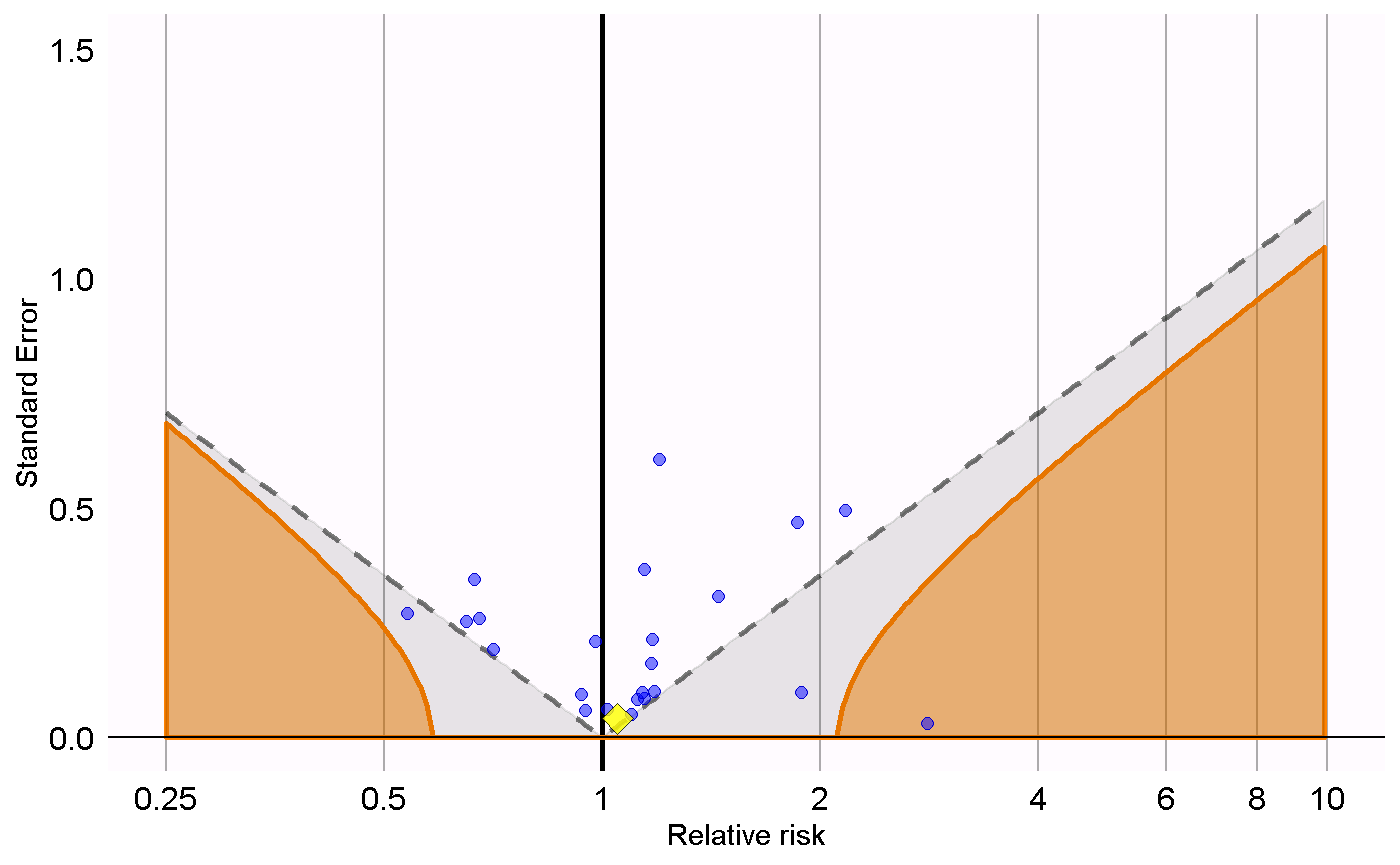
\includegraphics{../inst/doc/MultipleAnalyses_files/figure-latex/unnamed-chunk-17-1.pdf}

\begin{Shaded}
\begin{Highlighting}[]
\CommentTok{# Analysis 2: Nesting in rheumatoid arthritis}
\NormalTok{negCons <-}\StringTok{ }\NormalTok{analysisSum[analysisSum}\OperatorTok{$}\NormalTok{analysisId }\OperatorTok{==}\StringTok{ }\DecValTok{2} \OperatorTok{&}\StringTok{ }\NormalTok{analysisSum}\OperatorTok{$}\NormalTok{exposureId }\OperatorTok{!=}\StringTok{ }\DecValTok{1124300}\NormalTok{, ]}
\NormalTok{ei <-}\StringTok{  }\NormalTok{analysisSum[analysisSum}\OperatorTok{$}\NormalTok{analysisId }\OperatorTok{==}\StringTok{ }\DecValTok{2} \OperatorTok{&}\StringTok{ }\NormalTok{analysisSum}\OperatorTok{$}\NormalTok{exposureId }\OperatorTok{==}\StringTok{ }\DecValTok{1124300}\NormalTok{, ]}
\NormalTok{null <-}\StringTok{ }\KeywordTok{fitNull}\NormalTok{(negCons}\OperatorTok{$}\NormalTok{logRr, negCons}\OperatorTok{$}\NormalTok{seLogRr)}
\KeywordTok{plotCalibrationEffect}\NormalTok{(}\DataTypeTok{logRrNegatives =}\NormalTok{ negCons}\OperatorTok{$}\NormalTok{logRr, }
                      \DataTypeTok{seLogRrNegatives =}\NormalTok{ negCons}\OperatorTok{$}\NormalTok{seLogRr, }
                      \DataTypeTok{logRrPositives =}\NormalTok{ ei}\OperatorTok{$}\NormalTok{logRr, }
                      \DataTypeTok{seLogRrPositives =}\NormalTok{ ei}\OperatorTok{$}\NormalTok{seLogRr, }
\NormalTok{                      null)}
\end{Highlighting}
\end{Shaded}

\begin{verbatim}
#> Warning in fitNull(negCons$logRr, negCons$seLogRr): Estimate(s) with NA
#> standard error detected. Removing before fitting null distribution
\end{verbatim}

\begin{verbatim}
#> Warning: Removed 10 rows containing missing values (geom_point).
\end{verbatim}

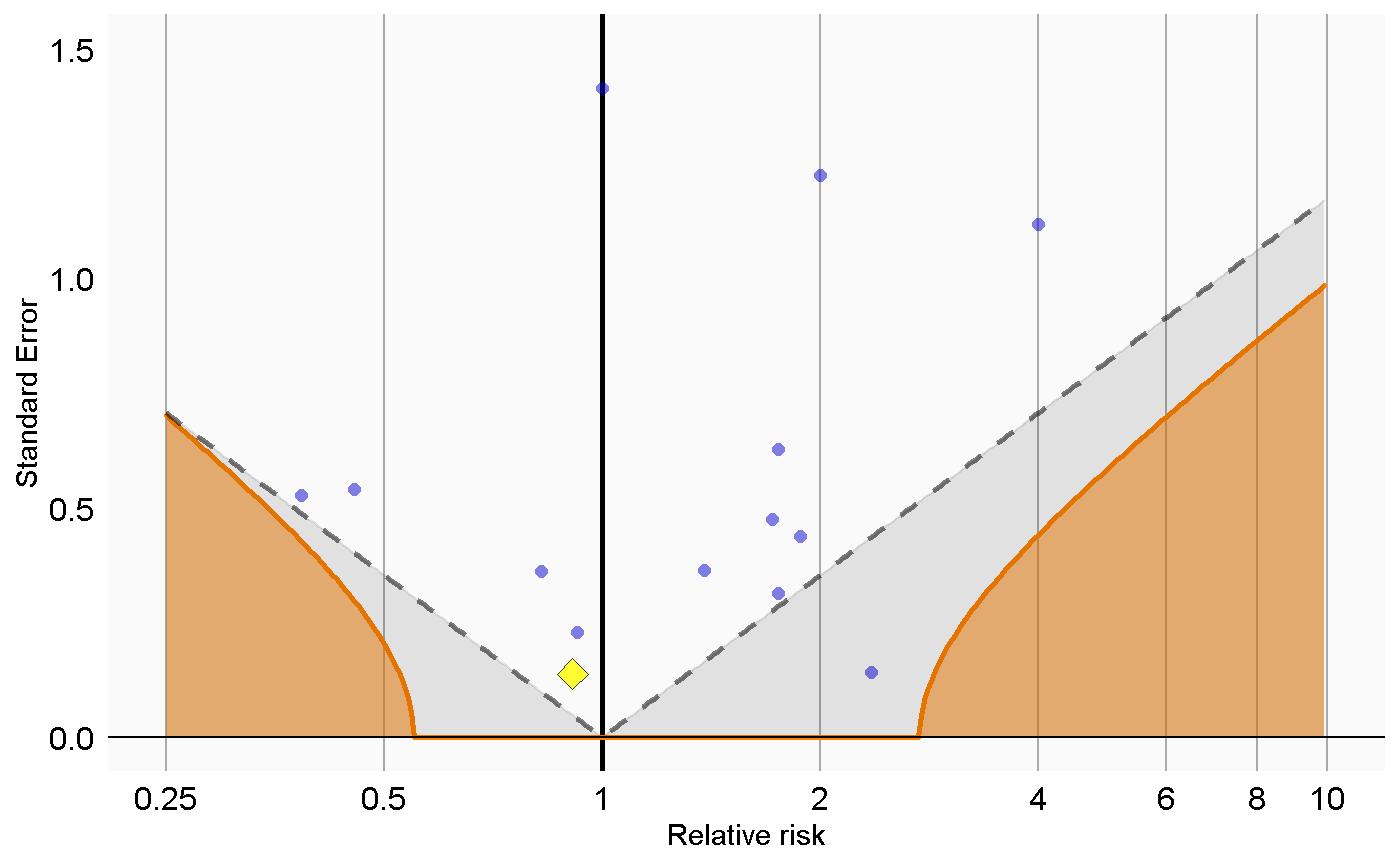
\includegraphics{../inst/doc/MultipleAnalyses_files/figure-latex/unnamed-chunk-19-1.pdf}

\begin{Shaded}
\begin{Highlighting}[]
\CommentTok{# Analysis 3: Nested case-time-control, matching on age and gender}
\NormalTok{negCons <-}\StringTok{ }\NormalTok{analysisSum[analysisSum}\OperatorTok{$}\NormalTok{analysisId }\OperatorTok{==}\StringTok{ }\DecValTok{3} \OperatorTok{&}\StringTok{ }\NormalTok{analysisSum}\OperatorTok{$}\NormalTok{exposureId }\OperatorTok{!=}\StringTok{ }\DecValTok{1124300}\NormalTok{, ]}
\NormalTok{ei <-}\StringTok{  }\NormalTok{analysisSum[analysisSum}\OperatorTok{$}\NormalTok{analysisId }\OperatorTok{==}\StringTok{ }\DecValTok{3} \OperatorTok{&}\StringTok{ }\NormalTok{analysisSum}\OperatorTok{$}\NormalTok{exposureId }\OperatorTok{==}\StringTok{ }\DecValTok{1124300}\NormalTok{, ]}
\NormalTok{null <-}\StringTok{ }\KeywordTok{fitNull}\NormalTok{(negCons}\OperatorTok{$}\NormalTok{logRr, negCons}\OperatorTok{$}\NormalTok{seLogRr)}
\KeywordTok{plotCalibrationEffect}\NormalTok{(}\DataTypeTok{logRrNegatives =}\NormalTok{ negCons}\OperatorTok{$}\NormalTok{logRr, }
                      \DataTypeTok{seLogRrNegatives =}\NormalTok{ negCons}\OperatorTok{$}\NormalTok{seLogRr, }
                      \DataTypeTok{logRrPositives =}\NormalTok{ ei}\OperatorTok{$}\NormalTok{logRr, }
                      \DataTypeTok{seLogRrPositives =}\NormalTok{ ei}\OperatorTok{$}\NormalTok{seLogRr, }
\NormalTok{                      null)}
\end{Highlighting}
\end{Shaded}

\begin{verbatim}
#> Warning in fitNull(negCons$logRr, negCons$seLogRr): Estimate(s) with NA
#> standard error detected. Removing before fitting null distribution
\end{verbatim}

\begin{verbatim}
#> Warning: Removed 15 rows containing missing values (geom_point).
\end{verbatim}

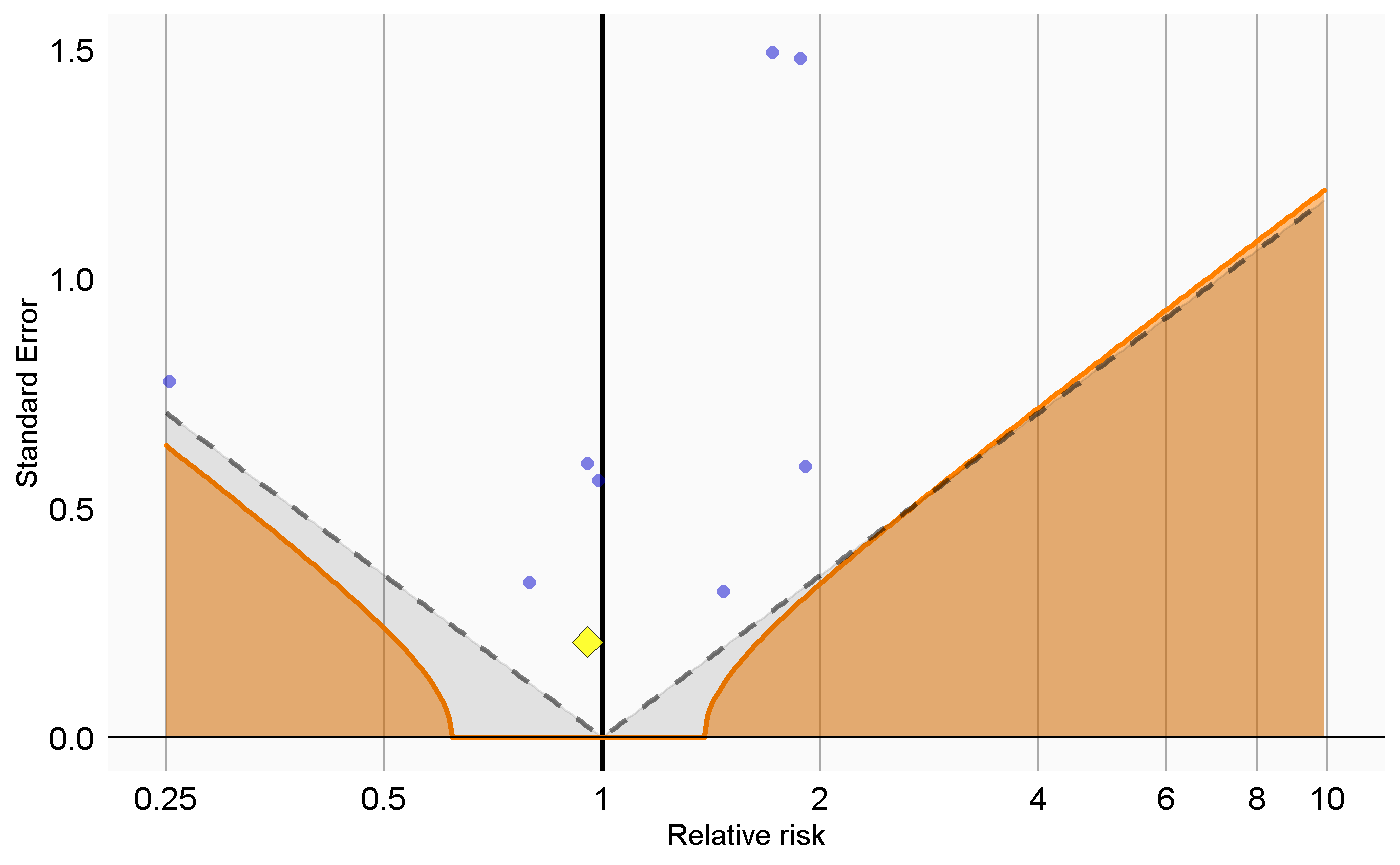
\includegraphics{../inst/doc/MultipleAnalyses_files/figure-latex/unnamed-chunk-21-1.pdf}

\begin{Shaded}
\begin{Highlighting}[]
\CommentTok{# Analysis 4: Nested case-time-control, matching on age, gender, and visit}
\NormalTok{negCons <-}\StringTok{ }\NormalTok{analysisSum[analysisSum}\OperatorTok{$}\NormalTok{analysisId }\OperatorTok{==}\StringTok{ }\DecValTok{4} \OperatorTok{&}\StringTok{ }\NormalTok{analysisSum}\OperatorTok{$}\NormalTok{exposureId }\OperatorTok{!=}\StringTok{ }\DecValTok{1124300}\NormalTok{, ]}
\NormalTok{ei <-}\StringTok{  }\NormalTok{analysisSum[analysisSum}\OperatorTok{$}\NormalTok{analysisId }\OperatorTok{==}\StringTok{ }\DecValTok{4} \OperatorTok{&}\StringTok{ }\NormalTok{analysisSum}\OperatorTok{$}\NormalTok{exposureId }\OperatorTok{==}\StringTok{ }\DecValTok{1124300}\NormalTok{, ]}
\NormalTok{null <-}\StringTok{ }\KeywordTok{fitNull}\NormalTok{(negCons}\OperatorTok{$}\NormalTok{logRr, negCons}\OperatorTok{$}\NormalTok{seLogRr)}
\KeywordTok{plotCalibrationEffect}\NormalTok{(}\DataTypeTok{logRrNegatives =}\NormalTok{ negCons}\OperatorTok{$}\NormalTok{logRr, }
                      \DataTypeTok{seLogRrNegatives =}\NormalTok{ negCons}\OperatorTok{$}\NormalTok{seLogRr, }
                      \DataTypeTok{logRrPositives =}\NormalTok{ ei}\OperatorTok{$}\NormalTok{logRr, }
                      \DataTypeTok{seLogRrPositives =}\NormalTok{ ei}\OperatorTok{$}\NormalTok{seLogRr, }
\NormalTok{                      null)}
\end{Highlighting}
\end{Shaded}

\begin{verbatim}
#> Warning in fitNull(negCons$logRr, negCons$seLogRr): Estimate(s) with NA
#> standard error detected. Removing before fitting null distribution
\end{verbatim}

\begin{verbatim}
#> Warning: Removed 14 rows containing missing values (geom_point).
\end{verbatim}

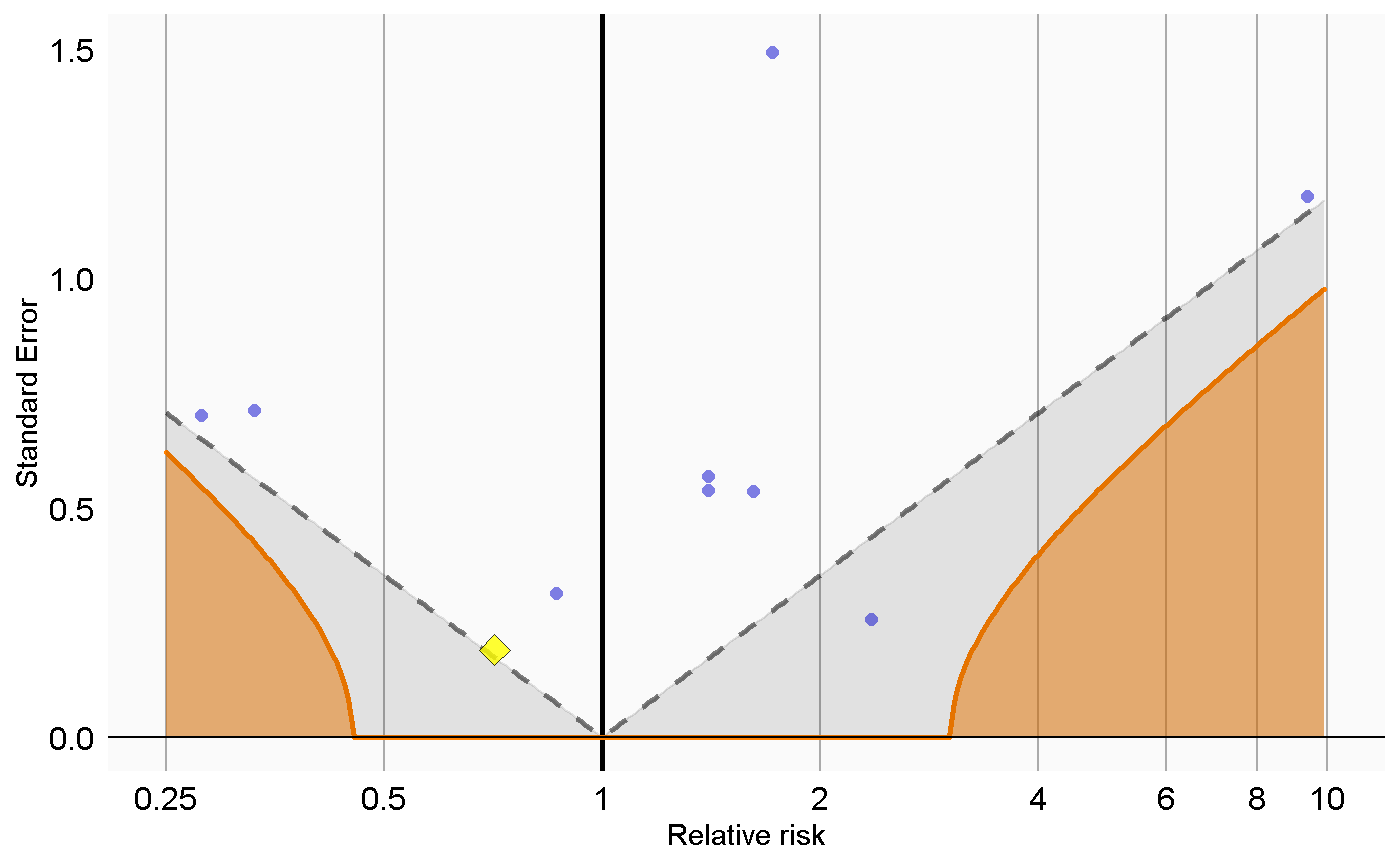
\includegraphics{../inst/doc/MultipleAnalyses_files/figure-latex/unnamed-chunk-23-1.pdf}
\#\# Acknowledgments

Considerable work has been dedicated to provide the
\texttt{CaseCrossover} package.

\begin{Shaded}
\begin{Highlighting}[]
\KeywordTok{citation}\NormalTok{(}\StringTok{"CaseCrossover"}\NormalTok{)}
\end{Highlighting}
\end{Shaded}

\begin{verbatim}
#> 
#> To cite package 'CaseCrossover' in publications use:
#> 
#>   Martijn Schuemie (2018). CaseCrossover: Case-Crossover. R
#>   package version 1.1.0. https://github.com/OHDSI/CaseCrossover
#> 
#> A BibTeX entry for LaTeX users is
#> 
#>   @Manual{,
#>     title = {CaseCrossover: Case-Crossover},
#>     author = {Martijn Schuemie},
#>     year = {2018},
#>     note = {R package version 1.1.0},
#>     url = {https://github.com/OHDSI/CaseCrossover},
#>   }
\end{verbatim}

Further, \texttt{CaseCrossover} makes extensive use of the
\texttt{Cyclops} package.

\begin{Shaded}
\begin{Highlighting}[]
\KeywordTok{citation}\NormalTok{(}\StringTok{"Cyclops"}\NormalTok{)}
\end{Highlighting}
\end{Shaded}

\begin{verbatim}
#> 
#> To cite Cyclops in publications use:
#> 
#> Suchard MA, Simpson SE, Zorych I, Ryan P, Madigan D (2013).
#> "Massive parallelization of serial inference algorithms for
#> complex generalized linear models." _ACM Transactions on Modeling
#> and Computer Simulation_, *23*, 10. <URL:
#> http://dl.acm.org/citation.cfm?id=2414791>.
#> 
#> A BibTeX entry for LaTeX users is
#> 
#>   @Article{,
#>     author = {M. A. Suchard and S. E. Simpson and I. Zorych and P. Ryan and D. Madigan},
#>     title = {Massive parallelization of serial inference algorithms for complex generalized linear models},
#>     journal = {ACM Transactions on Modeling and Computer Simulation},
#>     volume = {23},
#>     pages = {10},
#>     year = {2013},
#>     url = {http://dl.acm.org/citation.cfm?id=2414791},
#>   }
\end{verbatim}

This work is supported in part through the National Science Foundation
grant IIS 1251151.


\end{document}
